\documentclass{article}
\usepackage{graphicx} % Required for inserting images
\usepackage{amsmath}
\title{N^2 queens}
\usepackage{amsmath,amsfonts,amsthm} % Math packages
\usepackage{amssymb}
\usepackage{mathtools}
\usepackage{float}
\author{Louis Larcher, Zacharie Perego, Rudolf Yazbeck}
\date{December 2025}

\begin{document}

\maketitle

\section{MCMC simulation}

\subsection{Defining the state space}
Let $x =(x_{(i,j,k)} \in \{0,+1\}: (i,j,k) \in \{ 1,2,...,N\}^3)$ be the 3D grid where each cell takes values 0 or 1, we define the state space S as all such elements that have $N^2$ non-zero elements exactly. 
\newline
The cube $x_{(i,j,k)}$ has value 0 assigned to it if there is no queen on it, and takes value 1 if there is a queen.

\subsection{Energy function design}
Our energy function H takes as input the state of the 3D chess board, returns value 0 when no two queens attack each other, and positive values otherwise. To do this, we check for each queen if she is facing another queen on one of the i, j or k axes or on the 2D or 3D diagonals. Please note that when we say that two queens are "attacking each other" we ignore intermediary queens that could be blocking the attack\newline 
We picked this energy function because it allows the algorithm to have a lower probability of accepting a transition to a state that has more queens attacking each other, and we ignore intermediary queens for two reasons: firstly, it makes sense to differentiate the cases where there are only two queens on a same axis and N queens on the same axis (we prefer the former), and secondly because it allows the algorithm's energy function computation to be optimized based on the previous state, more on this below.
\newline 
\newline 
Let us first define rigorously what each type of attack is defined as. Let $q_1$ be a queen, i.e. an element of $x$ such that its coordinates are $(i_1, j_1, k_1)$ and let $q_2$ be a separate queen such that its coordinates are $(i_2, j_2, k_2)$. The different conditions for an attack are defined as follows: \newline

For the queens to be attacking each other on the same axis the condition is sharing exactly two coordinates: \newline
$i_1 = i_2 \ \& \ j_1=j_2$ or $i_1 = i_2 \ \& \ k_1 = k_2$ or $j_1 = j_2 \ \& \ k_1 = k_2$ \ \newline
There are 3 such axes.\newline \newline
On the 2D diagonals the conditions for an attack are : \newline
On the $(i,j)$ plane : 
$$\vert i_1 - i_2 \vert = \vert j_1 - j_2\vert \quad \text{if} \ k_1 = k_2$$
On the $(i,k)$ plane : 
$$\vert i_1 - i_2 \vert = \vert k_1 - k_2\vert \quad \text{if} \ j_1 = j_2$$
On the  $(j,k)$ plane :
$$\vert j_1 - j_2 \vert = \vert k_1 - k_2\vert \quad \text{if} \ i_1 = i_2$$ 
Our queen is in a 3D space and we care about 2D diagonals, so for those she can move in one of $\binom{3}{2}=3$ 2D planes, meaning we have 6 possible 2D diagonals to move in.
\newline \newline
On the 3D diagonals the condition is : $$\vert i_1 - i_2 \vert = \vert j_1 - j_2 \vert = \vert k_1 - k_1 \vert > 0$$ 
Take the queen on the cube with coordinates $(x,y,z)$. The possible moves on the 3D diagonals are $(x \pm 1, y \pm 1, z \pm 1)$, meaning there are $\frac{2^3}{2}=4$ 3D diagonals to move in because we have to fix one of the signs. \newline 

Let us also define the indicator function that indicates if two given queens are attacking each other, i.e. fulfill any of the conditions above 
$$
\mathbb{I}(q_1,q_2)=\begin{cases}
			1, & \text{if the queens are attacking each other}\\
            0, & \text{otherwise}
		 \end{cases}
$$
\newline 
We define for a given state $x \in S$ the energy function:
\newline
\begin{align*}
H(x) = \sum_{q_1 \in x : q_1=1}{} \sum_{q_2 \in x: q_2=1,q_2 \neq q_1}{\mathbb{I}(q_1,q_2)}
\end{align*}
A double sum has to be done in order to compute H, but we came up with an optimization to change the value based on the last state and not check if each queen is being attacked at O($N^4$) rather than O($N$).

The algorithm to compute the heat function is the following: \newline 
Let $G=(V,E)$ be the graph where each of the $N^2$ queens is a node, and they are connected by an edge if and only if they are in an attacking position. The graph takes time O($N^2$) to construct, but that is done only once and is not taken into account when re-computing the energy function. When we move a chosen queen $q_1$ into a new position that is not occupied by another queen remove all edges connected to its corresponding vertex in O(1) time (and store the number of edges removed), then scan all axes, 3D and 2D diagonals in O(N) time, and keep a list of the queens that match this position all in O(N) if we assume the queens are stored in a hash-map. Then, for each element $q'$ of the list, add an edge connecting $(q,q')$ to $E$ in O(N) time. Now compute the difference between number of edges removed and number of edges added, and add this value (that can be either positive or negative) to H, this is the energy function of our new state.
\subsection{Monte-Carlo Markov chain design}
Let $x$ and $y$ be elements of S, we define the relation $x \sim y$ as the states $x$ and $y$ have all but one or no queens in the same positions. \newline
As an additional optimization, since the 2D (i,j) plane has $N^2$ squares and we have $N^2$ queens that aren't supposed to be attacking each other on an axis. By the pigeon hole principle, we will have to place exactly one queen on each cell of the 2D grid, otherwise there will be two superposed queens that will be attacking each other. Thus we will not get stuck in a local minimum if we fix each queen to a single cell and only move it along the k-axis, which will considerably reduce the convergence time for the algorithm.

We construct the base chain: $$\psi_{x,y}=\begin{cases}
			\frac{1}{N^2} \frac{1}{N} , & \text{if $x \sim y, x \neq y$ }\\
            \frac{1}{N}, & \text{if $x=y$} \\
            0, & \text{otherwise}
		 \end{cases}$$ \newline 
Since we are trying to minimize an energy function, we decided to use the same acceptance probabilities as the ones seen in the lecture 10 notes as follows:
$$a_{xy}=\begin{cases}
			min(1,e^{-\beta(H(y)-H(x))}) , & \text{if $x \sim y, x \neq y$ } \\
            0, & \text{otherwise}
		 \end{cases}
$$
Where we picked $\beta = 4$ after experimenting with different values. (We show in questions 2.2 an optimization)

The constructed chain has transition probabilities 
$$p_{xy}=\begin{cases}
			\psi_{xy}a_{xy} , & \text{if $x \neq y$ } \\
            1-\sum_{z \neq x}{\psi_{xz}a_{xz}}, & \text{x=y}
		 \end{cases}$$

\section{Further tasks and questions}

\subsection{Question 1}
\begin{figure}[H]
    \centering
    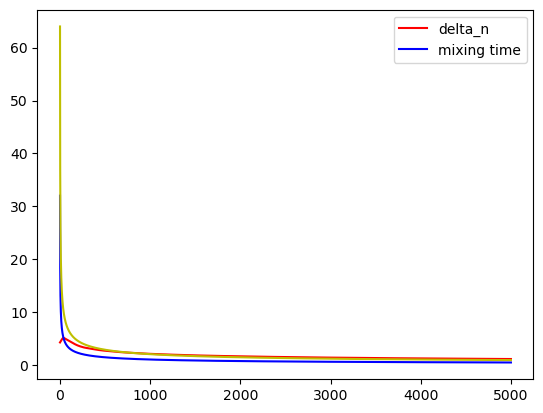
\includegraphics[width=0.5\linewidth]{output.png}
    \caption{Energy vs Steps, Beta=4, N=11}
    \label{fig:placeholder}
\end{figure}
\subsection{Question 2}
The use of a simulated annealing helps the algorithm converge faster and more reliably than with a fixed $\beta$. As plotted in Q1, only one simulation reached 0. 
We ran eight chains using parallel tempering with eight values of $\beta$ = [0.08, 0.2, 0.4, 0.7, 1.5, 3.5, 8.0, 12.0]. This allowed us to find a solution in 300'000 steps instead of $1 \cdot 10^6$. 

For readability reasons we only plotted one run, but all the runs we performed are quite similar in terms of convergence time. However, it is not always the same chain (among the eight) that converges.
 \begin{figure}[H]
    \centering
    \includegraphics[width=0.5\linewidth]{hjegdrfljhserdfg.png}
    \caption{Parallel Tempering Trace: Energy vs Steps (8 Replicas), Beta = [0.08, 0.2, 0.4, 0.7, 1.5, 3.5, 8.0, 12.0], N=11}
    \label{fig:placeholder}
\end{figure}

\subsection{Question 3}

\begin{figure}[H]
    \centering
    \includegraphics[width=0.5\linewidth]{image.png}
    \caption{Minimum energy reached vs N values}
    \label{fig:placeholder}
\end{figure}

\subsection{Question 4}
By optimizing the runtime, we can converge to a solution for relatively large values of $N$. No solution was found for $N \in \{1, 2, \ldots, 10, 12, 14\}$, but for $N \in \{11, 13\}$ we found
\[
\min_{x} H(x) = 0.
\]
\end{document}
